\documentclass[conference]{IEEEtran}
\IEEEoverridecommandlockouts
% The preceding line is only needed to identify funding in the first footnote. If that is unneeded, please comment it out.
\usepackage{cite}
\usepackage{amsmath,amssymb,amsfonts}
\usepackage{algorithmic}
\usepackage{graphicx}
\usepackage{multirow}
\usepackage{array}
\usepackage{textcomp}
\usepackage{xcolor}
\def\BibTeX{{\rm B\kern-.05em{\sc i\kern-.025em b}\kern-.08em
T\kern-.1667em\lower.7ex\hbox{E}\kern-.125emX}}
\begin{document}

\title{TaintBlade: A framework for automated protocol reverse engineering and study of botnet command and control protocols
}

\author{\IEEEauthorblockN{1\textsuperscript{st} Given Name Surname}
    \IEEEauthorblockA{\textit{dept. name of organizatiosn (of Aff.)} \\
        \textit{name of organization (of Aff.)}\\
        City, Country \\
        email address or ORCID}
    \and
    \IEEEauthorblockN{2\textsuperscript{nd} Given Name Surname}
    \IEEEauthorblockA{\textit{dept. name of organization (of Aff.)} \\
        \textit{name of organization (of Aff.)}\\
        City, Country \\
        email address or ORCID}
}

\maketitle

\begin{abstract}
    TODO redact this at the end
\end{abstract}

\begin{IEEEkeywords}
    TODO keywords
\end{IEEEkeywords}

\section{Introduction}
TODO - This section introduces the problem we are dealing with and motivates
the creation of this tool

%%%%%%%%%
- Mention here the evolution of botnets towards http and similar from custom protocols.
%%%%%%%%%

\section{Background}

TODO - This section goes over the state of the art on analyzing malware
binaries, past work on protocol reverse engineering and available tools.

%%%%%%%%%%%
\subsection{Automated protocol reverse engineering}
- Talk about what it is a protocol, and how to extract it.

- Mention dynamic analysis vs static ones (e.g. from packet traces).

- Talk about protocol message format inference vs state machine inference.

- Keywords, delimeters, pointer fields.

\subsection {Taint analysis}
- Talk about tainting, goals and how it works in general terms.
%%%%%%%%%%%

\section{Design}
TODO - This section covers the general structure of the tool and the different
modules and functionalities implemented.

- Requirements: overview and goals of the tool
- Arch: overview and details of each stage
- Implementation, with repo and how to use

\

In the previous sections, we introduced the issue of automating protocol
reverse engineering and the relevance of this task in the context of the
analysis of malware transmitting malicious communications. In this section, we
will now describe the automated protocol reverse engineering framework, called
\textit{TaintBlade}, that we have developed for tackling this task. Overall,
this tool pursues three main goals: (1) to perform message inference of the
underlying ingress protocol of a program, offering an accurate representation
of its compounding fields and the purpose of each byte; (2) to provide a
complete trace of the activities carried out by the instrumented program,
including a viewpoint into loaded images, child processes, executed routines
and their arguments, therefore helping the analyst with the reversing task,
rathering than just offering a black-box tool; (3) to become a framework usable
not only by malware analysts by offering specific functionalities aimed for
studying malware behaviours, but also by the general public by providing an
intuitive and fully enriched graphical user interface that offers additional
features and enhances cohesion over the data produced by the tool.

\subsection{Architecture overview}

\begin{figure}[htbp]
    \centerline{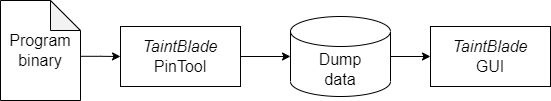
\includegraphics[width=0.9\columnwidth]{images/generalarch.drawio.png}}
    \caption{Example of a figure caption.}
    \label{fig_3_generalarch}
\end{figure}

From a general viewpoint, the functioning of \textit{TaintBlade} is, as shown
in figure \ref{fig_3_generalarch}: (1) the user selects a binary (an
executable) to be traced; (2) the program is executed and instrumented by
\textit{Intel PIN}, using \textit{TaintBlade} as a pintool, which reverses the
protocol of the program; (3) the pintool generates a set of output
\textit{.dfx} dump files and/or a SQLite database with all traced data; (4) the
user can navigate the resulting data by means of \textit{TaintBlade} GUI, which
interacts with the database, or by accessing the output dump files.

The \textit{TaintBlade} pintool is the central component of the framework. It
encompasses all the necessary instrumentation and tracing functionalities
required for the protocol reverse engineering task. At its core, the pintool
utilizes Intel PIN, which provides the instrumentation capabilities. On top of
Intel PIN, \textit{TaintBlade} features a series of \textit{modules} -
collections of components centered on a specific stage of the protocol reverse
engineering task or that offer other additional functionalities intended to
facilitate malware reversing.

As it can be observed in figure \ref{figure:fig_3_archdetailedsteps},
\textit{TaintBlade} comprises six different modules, namely (1) an
instrumentation module which enables the framework to hook on each loaded
image, executed routines and on unique instructions, and to access any register
or memory data; (2) a tainting module featuring a multi-color scheme, which
enables to track the propagation of data at a byte level inside the
instrumented program; (3) a heuristics module that matches executed
instructions with tainted data to a set of heuristics corresponding to specific
operations; (4) a protocol reversing module that constructs a full protocol
from the gathered heuristics; (5) a tracing module that enables to detect the
execution of routines, logging its arguments; (6) and an auxiliary NOPer module
that allows for skipping code sections and to manually modify the program state
at arbitrary points.

Although each module works independently from the others, most of them operate
in a pipeline fashion, where the input of one module depends on that of the one
directly preceeding it. In particular, the instrumentation, tainting,
heuristics and protocol reversing modules work sequentially towards the
protocol reversing task, whilst the tracing and NOPer modules work separately,
offering support features to the tool. We will now study each module
individually and describe how they work internally and the coordination between
them.

\begin{figure*}
    \centerline{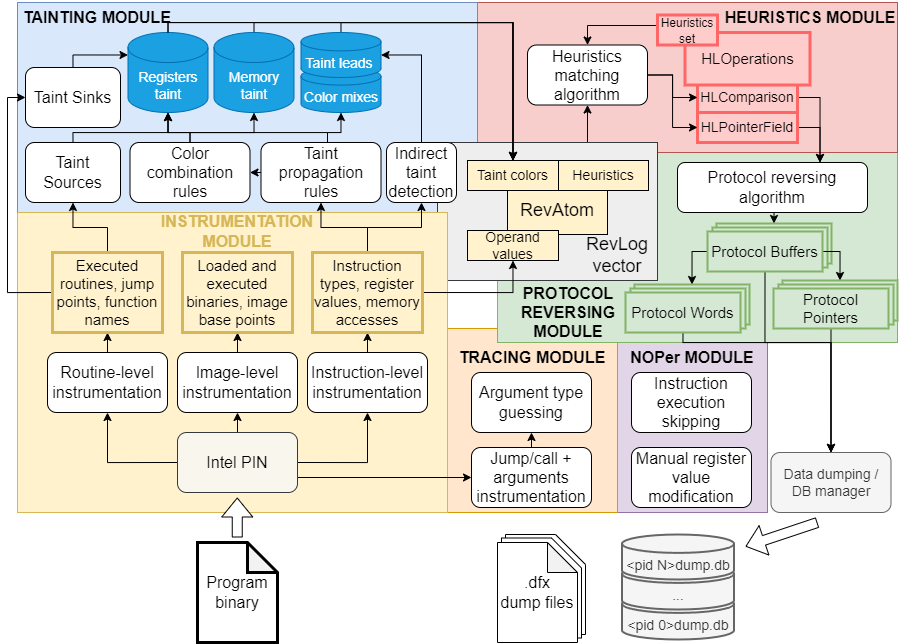
\includegraphics[width=\textwidth]{images/archdetailedsteps.drawio.png}}
    \caption{Example of a figure caption.}
    \label{figure:fig_3_archdetailedsteps}
\end{figure*}

\subsection{Instrumentation module}
The instrumentation module is the central component in the \textit{TaintBlade}
framework and the one that works closer to the assembly code. It utilizes Intel
PIN to instrument the program that is being executed at a triple level:
creating hooks for every loaded program image (e.g. an imported DLL), for every
executed routine (e.g. the \textit{main} function at the program) and for every
executed instruction (e.g. a single call instruction to some other function).

\textbf{Image instrumentation.}
\textit{TaintBlade} only instruments the instructions and routines that are included
in a list known as the \textit{image scope}. This scope is, by default, the main image of the executable
selected to be traced, although the user may select more images to be included via the GUI or
the program configuration files. By instrumenting program images, \textit{TaintBlade} informs the
user of when a new image is loaded - which may be of interest to the user, choosing it to be included
in the scope. This instrumentation also acts as support to other modules - like the NOPer module -, by calculating in
advance the virtual addresses of key instructions (such as those selected by the user to be manually skipped).

\textbf{Routine instrumentation.}
\textit{TaintBlade} instruments any newly executed routine included in the image scope. The instrumentation is double: it instruments
the routine right after it is called and before it returns. This enables
the tool to extract information such as the function and image names, and the memory address of the arguments with which each
function is called and with which it returns. Instrumenting routines is key for supporting the rest of the modules, and it is done in two different ways:

\begin{itemize}
    \item Comparing the name and image of the routine with an internal list of routines.
          The instrumentation of these routines is hardcoded, and therefore the tool
          knows exactly how to parse each of its arguments (the data structures each one
          corresponds to). This type of instrumentation is used from the tainting module,
          which needs to access specific data points in each routine at an specific time
          (either before or after the execution).
    \item Performing a more general instrumentation, without hardcoding the data types.
          As we will explain in section \ref{?}, this is useful for the tracing module,
          which will also attempt to guess the type of arguments later.
\end{itemize}

\textbf{Instruction instrumentation.}
This is the most important instrumentation type since it is the entrypoint for the tainting functionality.
Here \textit{TaintBlade} will examine each executed instruction individually, and
compare it with a list of instructions that the tool is prepared to work with. Table \ref{table:instruction_types_instrumentation_supported}
covers the instruction types currently supported by \textit{TaintBlade}. It must be noted that, for this version of the tool, we have focused
on supporting those instructions that we considered to be more commonly generated by compilers (and thus
more commonly found at any program). Certain instructions (like SHR, REPNE SCAS), although seemingly arbitrary,
often take part at the implementation of common routines found at most programs, like \textit{strncmp()} and \textit{strlen()},
which is the reason they were selected to be instrumented.

\begin{table}[htbp]
    \caption{Instruction types for which instrumentation is supported}
    \begin{center}
        \begin{tabular}{|>{\centering\arraybackslash}p{2cm}|c|>{\centering\arraybackslash}p{3.5cm}|}
            \hline
            \textbf{Instruction type} & \textbf{Instruction} & \textbf{Description} \\
            \hline
            \multirow{2}{*}{\shortstack{Arithmetic                                  \\ operations}} & ADD & \multirow{2}{*}{\shortstack{Any addition of memory,\\ immediate or register operands}}\\
                                      & SUB                  &                      \\
            \hline
            \multirow{3}{*}{\shortstack{Logical                                     \\ operations}} & AND & \multirow{3}{*}{\shortstack{Any logical operation\\ between memory, immediate\\ or register operands}}\\
                                      & OR                   &                      \\
                                      & XOR                  &                      \\
            \hline
            \multirow{6}{*}{\shortstack{Shift                                       \\ operations}} & \multirow{6}{*}{SHR} & \multirow{6}{*}{\shortstack{Shifting X number of bits\\ from a register to the right.\\Supports shifts of multiples\\of 8, since tainting module\\runs byte-based tracking.}}\\
                                      &                      &                      \\
                                      &                      &                      \\
                                      &                      &                      \\
                                      &                      &                      \\
                                      &                      &                      \\
            \hline
            \multirow{2}{*}{\shortstack{Comparison                                  \\ operations}} &  \multirow{2}{*}{CMP} & \multirow{2}{*}{\shortstack{Comparison between memory,\\ immediate or register operands}}\\
                                      &                      &                      \\
            \hline
            \multirow{4}{*}{\shortstack{Data moving                                 \\ operations}} & MOV & \multirow{4}{*}{\shortstack{Move values between memory,\\ immediate or register operands.}}\\
                                      & MOVSX                &                      \\
                                      & MOVSXD               &                      \\
                                      & MOVZX                &                      \\
            \hline
            \multirow{3}{*}{\shortstack{Address moving                              \\ operations}} & \multirow{3}{*}{LEA}                  &   \multirow{3}{*}{\shortstack{Moving a pointer, all types\\ of LEA operands supported}}                     \\
                                      &                      &                      \\
                                      &                      &                      \\
            \hline
            \multirow{5}{*}{\shortstack{Control flow                                \\ instructions}} & CALL& \multirow{5}{*}{\shortstack{Any jump, call or return.\\ Supported both near and far\\ relative displacement types}}\\
                                      & JMP                  &                      \\
                                      & JB                   &                      \\
                                      & JBE                  &                      \\
                                      & RET                  &                      \\
            \hline
            \multirow{5}{*}{\shortstack{String                                      \\ manipulation\\ operations}} & SCASB & \multirow{5}{*}{\shortstack{Instructions used for operating\\ with string types, supports\\ iterations with REPNE prefix}}\\
                                      & SCASD                &                      \\
                                      & SCASQ                &                      \\
                                      & SCASW                &                      \\
                                      & REPNE SCASX          &                      \\
            \hline
        \end{tabular}
        \label{tab1}
    \end{center}
    \label{table:instruction_types_instrumentation_supported}
\end{table}

When an instruction is instrumented, \textit{TaintBlade} first checks the type
of instruction by making use of the Intel XED decoder[?] that comes embedded in
Intel PIN. This decoder lets the tool classify the instruction, grouping it
with other instruction types that share the same properties (e.g. every
arithmetic operation is instrumented similarly). Once classified, the tool
analyzes the arguments of the instruction and extracts any needed addresses
and/or values from it. This data will be then used as an input for the tainting
functionality.

\subsection{Tainting module}
\textit{TaintBlade} features a custom multi-color tainting engine for the x86
and x86\_64 architectures, operating at the byte-level. The rationale for this is
that we needed to track and distinguish each byte received from a specific code program point.
By employing multiple colors, we can then gather key information regarding how these bytes
are combined between each other and how they are used inside the program.

This initial version of the tool is fully prepared to work in Windows systems,
although it could be easily extended to work in Linux in a future. It must also
be noted that we decided to develop the tainting system from the ground -
instead of using an existing solution - because we did not find any
implementation of a taint system for x86\_64 Windows machines that included
multi-color taint tracking. We considered well-known engines like libdtf,
Triton or Dytan but, as indicated in table
\ref{table:taining_engines_reason_not_chosen}, we identified certain drawbacks
in each of them.

\begin{table}[htbp]
    \caption{Existing open-source tainting engines, not selected}
    \begin{center}
        \begin{tabular}{|>{\centering\arraybackslash}p{1.5cm}|c|>{\centering\arraybackslash}p{3.5cm}|}
            \hline
            \textbf{Engine}         & \textbf{Characteristics} & \textbf{Drawbacks}                                      \\
            \hline
            \multirow{3}{*}{libdft} & Linux x86                & \multirow{3}{*}{\shortstack{No Windows, x86\_64 support \\ Limited number of colors}}\\
                                    & Multi-color              &                                                         \\
                                    & (max. 8 colors)          &                                                         \\
            \hline
            \multirow{2}{*}{\shortstack{libdft64                                                                         \\ (Angora)}} & Linux x86\_64 & \multirow{2}{*}{\shortstack{No Windows support\\Multi-color not supported}}\\
                                    & Mono-color               &                                                         \\
            \hline
            \multirow{2}{*}{Dytan}  & Linux x86                & \multirow{2}{*}{\shortstack{No windows, x86\_64 support \\ Multi-color not supported}}\\
                                    & Mono-color               &                                                         \\
            \hline
            \multirow{4}{*}{Triton} & Windows, Linux           & \multirow{4}{*}{\shortstack{Multi-color not supported}} \\
                                    & x86, x86\_64,            &                                                         \\
                                    & ARM32, AArch64           &                                                         \\
                                    & Mono-color               &                                                         \\
            \hline
        \end{tabular}
        \label{tab1}
    \end{center}
    \label{table:taining_engines_reason_not_chosen}
\end{table}

We would like to highlight the difficulty of modifying these existing systems
to support our purposes. Adapting an engine to a new architecture requires
creating new taint rules for the new Instruction Set Architecture (ISA).
Moreover, moving from a 32-bit-sized architecture to a 64-bit-sized one
involves additional challenges. One of them is that tainting engines in the x86
architecture usually feature (like in libdft) a shadow memory with the same
size as that of the whole virtual address space (limited to $2^{32}$ bytes in
x86), which tracks the taint state of each byte. This is completely unfeasible
to do in a 64-bit system, since the virtual address space can be up to $2^{64}$
(although processor implementations may reduce this value
\cite{book_practical_binary_analysis_p13}).

Another challenge is the implementation of multi-color taint tracking in a
mono-color system. The introduction of one of such systems involves changing
the taint storage from a bitmap value, where 0=not tainted and 1=tainted, to a
data structure that supports multiple values, together with all taint
propagation policies in order to support this change. Additionally, we would
find that the number of possible colors is limited to the capacity of the
structure previously used.

Therefore, taking all the previous into account, we decided to create our own
completely new 64-bit-compatible multi-color tainting engine that integrates
with Intel PIN (it relies on the instrumentation module we described
previously).

\textbf{Taint storage.} The tainting module keeps a centralized set
of data structures that store the taint information of the registers and memory of
a single instrumented process.
Since \textit{TaintBlade} supports both the x86 and x86\_64 architectures, it is not feasiable to
maintain a shadow memory of the process with the color of each byte. Instead, we
achieved an optimized implementation that pursues two main goals:
\begin{itemize}
    \item Since we cannot shadow all memory in the process, we dynamically generate or
          destroy taint data at runtime, thus giving up on temporal optimization but
          allowing to taint any number of memory addresses.
    \item We expect that taint colors from tainted bytes are frequently combined during
          program execution. Therefore, we will support an arbitrary number of color
          combinations, improving the design described in section [??reference section
            showcasing libdft??].
\end{itemize}

Considering the goals described previously, the taint storage of our engine
follows the architecture shown in figure \ref{figure:taintingengine}. As it can
be observed, we dispose of two main structures, one for storing memory colors
and another for register colors. In the case of memory tainting, we store in an
unordered map pairs of data corresponding to each individual tainted memory
address and the color that it has been tainted with. This map is modified at
runtime, so that addresses not contained in the map are assumed not to be
tainted.

In the other hand, we will track the taint in each of the registers of the
process by means of a vector that acts as a shadow processor. In this vector,
we will contain one element for each byte of each register (including
\textit{rax}, \textit{rbx}, \textit{rcx}, \textit{rdx}, \textit{r8} ...
\textit{r15}, \textit{rsi}, \textit{rdi}, \textit{rsp} and \textit{rbp}). Each
element will hold the color with which an specific byte of that register has
been tainted. Note that a value of 0 means that the register byte is not
tainted. Also, support for the x86 architecture is guaranteed by, at runtime,
ignoring half the bytes for each register. We follow the same technique when
instrumenting a program that makes use of, for example, 8-byte registers like
\textit{al}, by only taking the last 8 bytes in the vector corresponding to
register \textit{rax}.

\begin{figure}
    \centerline{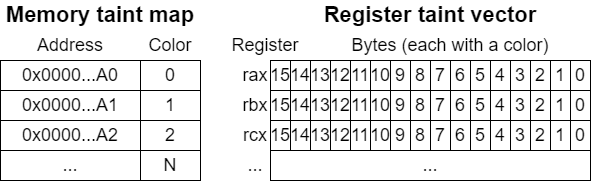
\includegraphics[width=0.9\columnwidth]{images/TaintingEngine.drawio.png}}
    \caption{Taint storage data structures.}
    \label{figure:taintingengine}
\end{figure}

\textbf{Multi-color support.} Although the previous architecture already allows
us to store our taint data, a multi-color engine requires additional data structures
for taint colors. During the program execution, taint colors will be generated
and combined to create new ones. These combinations, known as color mixes in
our engine, will need to be stored so that we can trackback which original colors
were combined to generate a certain derivate color.

The tainting module features the color mixes functionality by means of two
additional data structures. The current version of \textit{TaintBlade} supports
binary color mixes, meaning that any color is either original or the
combination of two other colors. As we will describe, the color mixes data
structures will need to be frequently accessed for two main purposes:
\begin{itemize}
    \item Knowing whether a certain color has been already generated as a result of the
          mix of two other colors.
    \item Getting the colors that were combined to generate a certain derivate color.
\end{itemize}

Therefore, we have developed the data structures that are detailed in figure
\ref{figure:colormixtaintarch}, consisting on two maps. The first map stores,
for each entry, a color that was generated as a mix of two other colors, and
the colors used in the mix. This is useful since we frequently need to access
whether a color mix has been generated already. In turn, the second map stores,
for each color, which colors it has been mixed with, and the result of the mix.
This is particularly needed for the case of getting the result of the mix of
two specific colors, since without an additional map we would need to traverse
the whole first color mix map.

\begin{figure}
    \centerline{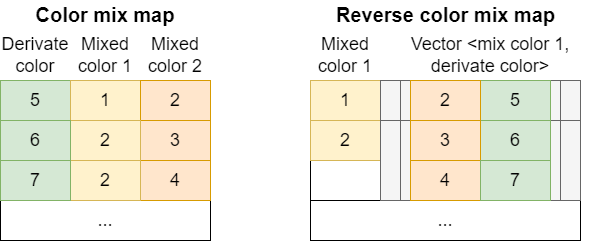
\includegraphics[width=0.9\columnwidth]{images/colormixtaintarch.drawio.png}}
    \caption{Taint storage data structures.}
    \label{figure:colormixtaintarch}
\end{figure}

\textbf{Taint sources.} Once considered how taint colors are stored in the tainting
module, we will discuss how these colors are generated in the first place. \textit{TaintBlade}'s
tainting module follows the architecture described in section \ref{}, by specifying taint sources
which generate the taint colors at specific registers and memory bytes.

In \textit{TaintBlade}, every taint source is a routine. A routine declared as
a taint source will perform the following actions:
\begin{enumerate}
    \item Using the instrumentation module, hook the routine before its execution and
          take the arguments with which it was called.
    \item Interpret the arguments received, casting them to the data structure that we
          know corresponds to them, previously hardcoded.
    \item Using the instrumentation module, hook the routine after its execution and the
          arguments with which the function returns.
    \item Again, cast the value of the arguments at the time of returning to the data
          structure that has been hardcoded.
    \item Depending on the routine, taint with different colors specific bytes of the
          arguments that have been either received or returned.
\end{enumerate}

Currently, \textit{TaintBlade} is focused on working with network protocols
and, therefore, the taint sources we have defined correspond to those routines
most commonly used for receiving network information. Table
\ref{table:taint_sources_and_taint_sinks} details the taint sources currently
implemented and which bytes get tainted when they are triggered. Note, however,
that these could be extended in the future to support any arbitrary routine.

\textbf{Taint sinks.} Just like we define program points at which to generate taint colors,
\textit{TaintBlade} also incorporates a series of routines acting as taint sinks,
at which we are interested to know whether any tainted data is received via the passed
arguments. In this initial version, we have incorporated three routines, detailed at
table \ref{table:taint_sources_and_taint_sinks}, that have are relevant for our protocol
reverse engineering task and perfom certain actions when triggered:
\begin{enumerate}
    \item CreateProcessA and CreateProcessW will receive a command to be executed. By
          defining them as taint sinks, we will be alerted whenever a tainted byte (that
          comes from the network) happens to be one of these commands.
    \item In Windows, due to historical reasons, many API calls are available either with
          ANSI strings in the arguments (taking \textit{char*}) or with UNICODE "wide"
          strings (as \textit{wchar\_t*}). MultiByteToWideChar is a function that allows
          us to convert strings between these two types, and it can thus be commonly
          found in programs. By defining this routine as taint sink, we are able not only
          to detect whether it receives tainted data, but also to transfer this data to
          the new, converted string, therefore ensuring we do not incur on undertainting.
\end{enumerate}

Whenever some taint color is found to reach a taint sink, that taint color is logged in an internal
vector, so that it can later be used when reversing the protocol.

\begin{table*}[htbp]
    \caption{Implemented taint sources and taint sinks in TaintBlade}
    \begin{center}
        \begin{tabular}{|c|>{\centering\arraybackslash}p{2.8cm}|>{\centering\arraybackslash}p{1.4cm}|>{\centering\arraybackslash}p{0.8cm}|c|>{\centering\arraybackslash}p{4cm}|}
            \hline
             & \multirow{2}{*}{\textbf{\shortstack{Routine                                                                                                                                                      \\name}}}                & \multirow{2}{*}{\textbf{DLL}} & \multirow{2}{*}{\textbf{Arch}} & \multirow{2}{*}{\textbf{Arguments}} & \multirow{2}{*}{\textbf{Taint actions}} \\
             &                                                                    &                               &                                 &  &                                                        \\
            \hline
            \multirow{10}{*}{\shortstack{\textbf{Taint}                                                                                                                                                         \\\textbf{sources}}}& \multirow{5}{*}{Recv$^{(\mathrm{a})}$} & \multirow{5}{*}{\shortstack{ws2\_32.dll                                          \\wsock32.dll }}  & \multirow{5}{*}{\shortstack{x86\\x86\_64}} &   \multirow{5}{*}{\shortstack{SOCKET s;\\char* buf;\\int len;\\int flags;}}      & \multirow{5}{*}{\shortstack{At exit, taints as many bytes\\from argument \textit{buf} as\\indicated in the return value.}}  \\
             &                                                                    &                               &                                 &  &                                                        \\
             &                                                                    &                               &                                 &  &                                                        \\
             &                                                                    &                               &                                 &  &                                                        \\
             &                                                                    &                               &                                 &  &                                                        \\
            \cline{2-6}
             & \multirow{5}{*}{\shortstack{InternetReadFile$^{(\mathrm{b})}$}}    & \multirow{5}{*}{wininet.dll}  & \multirow{5}{*}{\shortstack{x86                                                             \\x86\_64}}&    \multirow{5}{*}{\shortstack{LPVOID hFile;\\LPVOID lpBuffer;\\DWORD dwNumberOfBytesToRead;\\LPDWORD lpdwNumberOfBytesRead;}}      & \multirow{5}{*}{\shortstack{At exit, taints as many bytes\\from the argument \textit{lpBuffer} as\\indicated in argument\\\textit{lpdwNumberOfBytesRead}.}}\\
             &                                                                    &                               &                                 &  &                                                        \\
             &                                                                    &                               &                                 &  &                                                        \\
             &                                                                    &                               &                                 &  &                                                        \\
             &                                                                    &                               &                                 &  &                                                        \\
            \hline
            \hline
            \multirow{15}{*}{\shortstack{\textbf{Taint}                                                                                                                                                         \\\textbf{sinks}}}& \multirow{5}{*}{CreateProcessA$^{(\mathrm{c})}$} & \multirow{5}{*}{\shortstack{kernel32.dll}}  & \multirow{5}{*}{\shortstack{x86\\x86\_64}} &   \multirow{5}{*}{\shortstack{LPCSTR lpApplicationName;\\LPSTR lpCommandLine;\\LPSECURITY\_ATTRIBUTES lpProcessAttributes;\\(+7 other arguments)}}      & \multirow{5}{*}{\shortstack{Before executing the function,\\ it checks whether any byte from\\argument \textit{lpApplicationName}\\ is tainted.}}  \\
             &                                                                    &                               &                                 &  &                                                        \\
             &                                                                    &                               &                                 &  &                                                        \\
             &                                                                    &                               &                                 &  &                                                        \\
             &                                                                    &                               &                                 &  &                                                        \\
            \cline{2-6}
             & \multirow{5}{*}{\shortstack{CreateProcessW$^{(\mathrm{d})}$}}      & \multirow{5}{*}{kernel32.dll} & \multirow{5}{*}{\shortstack{x86                                                             \\x86\_64}}&    \multirow{5}{*}{\shortstack{LPCWSTR lpApplicationName;\\LPWSTR lpCommandLine;\\LPSECURITY\_ATTRIBUTES lpProcessAttributes;\\(+7 other arguments)}}     & \multirow{5}{*}{\shortstack{Before executing the function,\\ it checks whether any byte from\\argument \textit{lpApplicationName}\\ is tainted.}}  \\
             &                                                                    &                               &                                 &  &                                                        \\
             &                                                                    &                               &                                 &  &                                                        \\
             &                                                                    &                               &                                 &  &                                                        \\
             &                                                                    &                               &                                 &  &                                                        \\
            \cline{2-6}
             & \multirow{7}{*}{\shortstack{MultiByteToWideChar$^{(\mathrm{e})}$}} & \multirow{7}{*}{kernel32.dll} & \multirow{7}{*}{\shortstack{x86                                                             \\x86\_64}}&    \multirow{7}{*}{\shortstack{UINT CodePage;\\DWORD dwFlags;\\LPCCH lpMultiByteStr;\\int cbMultiByte;\\LPWSTR lpWideCharStr;\\int cchWideChar;}}     & \multirow{7}{*}{\shortstack{After executing the function,\\ take a byte \textit{i} from \textit{lpMultiByteStr}\\ and, if tainted, taint with the same\\ color the byte \textit{i} at \textit{lpWideChar},\\for a maximum of bytes indicated\\in the return value.}}  \\
             &                                                                    &                               &                                 &  &                                                        \\
             &                                                                    &                               &                                 &  &                                                        \\
             &                                                                    &                               &                                 &  &                                                        \\
             &                                                                    &                               &                                 &  &                                                        \\
             &                                                                    &                               &                                 &  &                                                        \\
             &                                                                    &                               &                                 &  &                                                        \\
            \hline
            \multicolumn{6}{l}{\shortstack{$^{(\mathrm{a})}$Routine and arguments defined following https://learn.microsoft.com/en-us/windows/win32/api/winsock/nf-winsock-recv}}                               \\
            \multicolumn{6}{l}{\shortstack{$^{(\mathrm{b})}$Routine and arguments defined following https://learn.microsoft.com/en-us/windows/win32/api/wininet/nf-wininet-internetreadfile}}                   \\
            \multicolumn{6}{l}{\shortstack{$^{(\mathrm{c})}$Routine and arguments defined following https://learn.microsoft.com/en-us/windows/win32/api/processthreadsapi/nf-processthreadsapi-createprocessa}} \\
            \multicolumn{6}{l}{\shortstack{$^{(\mathrm{d})}$Routine and arguments defined following https://learn.microsoft.com/en-us/windows/win32/api/processthreadsapi/nf-processthreadsapi-createprocessw}} \\
            \multicolumn{6}{l}{\shortstack{$^{(\mathrm{e})}$Routine and arguments defined following https://learn.microsoft.com/en-us/windows/win32/api/stringapiset/nf-stringapiset-multibytetowidechar}}      \\
        \end{tabular}
        \label{tab1}
    \end{center}
    \label{table:taint_sources_and_taint_sinks}
\end{table*}

\textbf{Taint propagation policy.} Once considered how taint colors are stored in the tainting
module, we will discuss how this data is propagated during the program execution. The goal of
the taint propagation policy is to define a set of rules that specify how taint colors are
moved across memory and registers depending on the instructions being executed. There exist
different rules, each corresponding to one of the instruction types we instrumented using the
instrumentation module and that we detailed at table \ref{table:instruction_types_instrumentation_supported}.
Note, however, that not all the instructions types incur in moving data, therefore only those
operating with data will have an attached taint rule.

\begin{table}[htbp]
    \caption{Taint rules for each instruction type}
    \begin{center}
        \begin{tabular}{|>{\centering\arraybackslash}p{2cm}|>{\centering\arraybackslash}p{5.5cm}|}
            \hline
            \textbf{Instruction type} & \textbf{Taint rule} \\
            \hline
            \multirow{3}{*}{\shortstack{Arithmetic          \\operations}} & \multirow{3}{*}{\shortstack{Mix destination operand colors using\\colors of source operand.}}\\
                                      &                     \\
                                      &                     \\
            \hline
            \multirow{4}{*}{\shortstack{Logical             \\operations}} & \multirow{4}{*}{\shortstack{If the operands are the same, untaint the\\operands. Otherwise, mix destination operand \\colors using colors of source operand.}}\\
                                      &                     \\
                                      &                     \\
                                      &                     \\
            \hline
            \multirow{5}{*}{\shortstack{Shift               \\operations}} & \multirow{5}{*}{\shortstack{Calculates the number of bytes shifted. Moves\\every color of every byte of the register to the\\right (from MSB to LSB). If the color goes\\out of bounds, the color is lost.}}\\
                                      &                     \\
                                      &                     \\
                                      &                     \\
                                      &                     \\
            \hline
            \multirow{4}{*}{\shortstack{Data moving         \\operations}}  & \multirow{4}{*}{\shortstack{Untaint the destination operand.\\Then, taint the destination operand with the\\colors from the source operand.}}\\
                                      &                     \\
                                      &                     \\
                                      &                     \\
            \hline
            \multirow{4}{*}{\shortstack{Address moving      \\operations}} & \multirow{4}{*}{\shortstack{Take colors of reg. leaBase and reg. leaIndex.\\Mix the colors with those of destination reg.\\Calculate indirect tainting.}}\\
                                      &                     \\
                                      &                     \\
                                      &                     \\
            \hline
            \multirow{6}{*}{\shortstack{String              \\ manipulation\\ operations}}  & \multirow{6}{*}{\shortstack{Take colors from memory being read. Mix them\\with colors of register \textit{al}, \textit{ax}, \textit{eax} or \textit{rax}\\depending on instruction length. Also, mix\\ them with colors of register \textit{di}, \textit{edi} or \textit{rdi}\\ depending on instruction length.}}\\
                                      &                     \\
                                      &                     \\
                                      &                     \\
                                      &                     \\
                                      &                     \\
            \hline
        \end{tabular}
        \label{tab1}
    \end{center}
    \label{table:taint_rules}
\end{table}

As detailed in the table, every taint rule results on either tainting,
untainting or mixing the colors of one or more operands:
\begin{itemize}
    \item If an operand gets tainted by another, it means that the colors of the
          destination operand get overwritten by those from the source operand.
    \item If an operand gets untainted, it means that its colors get removed, all set to
          0.
    \item If an operand gets mixed with another, it means that the colors of the
          destination operand get mixed, one by one, with those from the source operand.
\end{itemize}

Mixing colors consists on the following steps:
\begin{enumerate}
    \item Take the two colors to mix. Check in the reverse color mix map if that
          combination already exists.
          \begin{enumerate}
              \item If the color exists in the map, it means that the color mix has been produced
                    before. Therefore, the result of the mix is the previously generated mix color.
              \item If the color does not exist in the map, this is a new mix. Therefore, the
                    result of the mix is equal to the latest color mix produced + 1. (e.g. if the
                    last mix was color 5, then the new mix is color 6).
          \end{enumerate}
    \item Take the resulting mix color and log the mix in the mix maps.
\end{enumerate}

%%TODO DETAIL HERE INDIRECT TAINTING

\subsection{Heuristics module}
The previous two modules have instrumented the instructions and routines to
extract their arguments and operands, and also generated and propagated the
taint colors during its execution. However, in order to achieve our reverse
engineering task, we must be able to interpret the list of instrumented
instructions and their associated taint colors, so that we can eventually
extract the underlying operations that the program is performing with those
instructions. The heuristics module does exactly that. Its goal is to match
assembly instructions and taint data with the high-level operations the program
is performing. For instance, a sequence of \textit{cmp} assembly instructions
might indicate a program checking a buffer to have a certain value. In order to
achieve this matching, we perform the following process:

\textbf{Normalization.}
Firstly, \textit{TaintBlade} normalizes the available data by encapsulating the instruction information
extracted by the instrumentation module (the type of instruction, the value of the operands...) and the
taint colors of each operand indicated by the tainting module into an standard structure called a 'RevAtom'.
This RevAtom matches each operand values with the taint colors they have, and offer an abstraction
so that the heuristic module can operate with all data independently on the instruction type. In essence,
a RevAtom contains the following data:

\begin{enumerate}
    \item The instruction type.
    \item For every operand in the instruction, it contains:
          \begin{enumerate}
              \item The value of the operand.
              \item The taint color of the operand.
          \end{enumerate}
    \item Other optional data. This depends on the instruction type. For instance, for
          \textit{cmp} operations, we store the value of the RFLAGS register after the
          instruction execution, sot that we know if the comparison was successful. All
          optional data is gathered via the instrumentation module.
\end{enumerate}

Once a RevAtom is generated, \textit{TaintBlade} will check whether there
exists any operand in the RevAtom that holds a taint color. If every operand is
untainted, it means that, at a high-level, that instruction does not take part
in the management of tainted data, and thus has no relation to the underlying
protocol of the program. Therefore, if every operand is untainted, the RevAtom
is discarded. In the case that any operand is tainted, then we are interested
in examining that instruction further. In this case, the tool will introduce
the RevAtom in a centralized vector known as the 'RevLog'.

\textbf{Heuristic analysis}
Once we have a new RevAtom in the RevLog vector, \textit{TaintBlade} will try to match the RevAtoms in the RevLog
to a set of heuristics. A heuristic is an instruction, or a set of instructions, that define a high-level
operation happening in a program. In the previous example, a \textit{cmp} instruction where some of the operands
are tainted may indicate that the program is looking for some value in the tainted bytes, that is, from the data
received from the network (the taint sources). Therefore, in this case we would look in the RevLog for RevAtoms
containing a \textit{cmp} instruction type and some tainted operand.

As we explained in the introduction, our goal is to be able to perform protocol
message inference, detecting keywords, delimeters and pointer fields in the
protocol. In order to do this, we have developed the heuristics detailed on
table \ref{table:implemented_heuristics}. As it can be observed, there exists
two different heuristics, where the 'comparison operation' heuristic
corresponds to the program performing some comparison against a value, and the
'pointer operation' describes a value that was added to a pointer, so that it
now points to some other address, also belonging to a the tainted buffer.

\begin{table}[htbp]
    \caption{Implemented heuristics in TaintBlade}
    \begin{center}
        \begin{tabular}{|>{\centering\arraybackslash}p{1.5cm}|>{\centering\arraybackslash}p{6.3cm}|}
            \hline
            \textbf{Heuristic} & \textbf{Instructions}                                                 \\
            \hline
            \multirow{12}{*}{\shortstack{Comparison                                                    \\operation}} & \multirow{2}{*}{\shortstack{CMP(mem, imm), where mem is tainted.}}\\
                               &                                                                       \\
            \cline{2-2}
                               & \multirow{2}{*}{\shortstack{CMP(reg1, reg2), where reg1 is tainted.}} \\
                               &                                                                       \\
            \cline{2-2}
                               & \multirow{2}{*}{\shortstack{CMP(reg1, reg2), where reg2 is tainted.}} \\
                               &                                                                       \\
            \cline{2-2}
                               & \multirow{2}{*}{\shortstack{CMP(mem, reg), where mem is tainted.}}    \\
                               &                                                                       \\
            \cline{2-2}
                               & \multirow{2}{*}{\shortstack{CMP(reg, mem), where reg is tainted.}}    \\
                               &                                                                       \\
            \cline{2-2}
                               & \multirow{2}{*}{\shortstack{CMP(reg, imm), where reg is tainted.}}    \\
                               &                                                                       \\
            \hline
            \multirow{3}{*}{\shortstack{Pointer                                                        \\operation}} & \multirow{3}{*}{\shortstack{LEA(memDest, [leaBase+(leaIndex*leaScale)+leaDis]),\\where an indirect taint is detected.}}\\
                               &                                                                       \\
                               &                                                                       \\
            \hline
        \end{tabular}
        \label{tab1}
    \end{center}
    \label{table:implemented_heuristics}
\end{table}

In order to match the RevAtoms to the heuristics, the module runs a search
algorithm in the RevLog. In essence, this algorithm scans the RevLog, starting
from the last inserted instruction, and checks whether there is any combination
of instructions that match one of the heuristics. Note that, although this
version of \textit{TaintBlade} does not incorporate heuristics with multiple
instructions, the algorithm supports them already.

Once an heuristic is found, the module extracts it and inserts it in an
internal vector. The full algorithm and implementation details regarding how
the heuristic matching process can be consulted in ANNEX TODO.

\subsection{Protocol reversing module}
As we described, during the program execution \textit{TaintBlade} will
accumulate all found heuristics in an internal vector. The final step is to
interpret the operations described in the heuristics, grouping or discarding
them, so that we are able to reverse the underlying protocol. This process
happens only once the program has finished.

In \textit{TaintBlade}, a protocol consists of a series of protocol buffers,
where each one corresponds to a set of bytes received from the network in a
single call (e.g. the bytes received from the taint source InternetReadFile
would be included in a single buffer). In each of the protocol buffers, we will
find a list of associated protocol words, that include keywords and delimeters,
and protocol pointers fields. Additionally, each of the bytes in the buffer include
whether or not they were found to have reached some of the taint sinks.

In order to reverse the protocol, a custom algorithm is used. This algorithm combines
the knowledge about the chronological order of the RevAtoms, the taint sinks information and,
in the case of the comparison operations, the result of the comparisons.
The complete algorithm and process can be seen in ANNEX TODO. As a summary, it will take the 
heuristics and output the protocol and associated buffers. In these buffers, we can find the 
following word types:

\textbf{Delimeter.} A delimeter is found when multiple comparison operations against the same byte 
are found in a sequential manner for contiguous bytes of the buffer, either in an incrementing 
or decrementing order. For each byte, the algorithm will check that the result of the comparison
was unsuccessful, that is, that the value being checked against the byte at the buffer was not equal.

If we find that multiple comparison operations are checked sequentially, and that none succeed, then this
indicates that the program was looking for a value in the buffer, yet it failed to find it. In this case,
we will mark the delimeter as failed in the protocol, so that this event is reported. 

Otherwise, if there exists a series of unsuccessful comparison operations followed by a single successful comparison
operation using the same byte value, this indicates that the program found the delimeter it was looking for.

\textbf{Keyword.} Every comparison operation is marked as a keyword if it is not part of a delimeter. After that, 
keywords are joined if they occupy sequential positions in the buffer, that is, if the color of the final byte of
one keyword is the previous one to the initial color of the other, and if they happened in chronological order
(one comparison after the other).

Note that, sometimes, it is possible to find keywords of a single byte, where the comparison is unsuccessful, and which are 
unable to be joined to another keyword. Due to the nature of dynamic analysis, this is ann event that happens when
the program checks a keyword byte by byte instead of using, for instance, a common routine like \textit{strcmp()}.  
In this cases, \textit{TaintBlade} marks the byte as a keyword but highlights the fact that it is isolated so
that the user has the chance of investigating it further if wanted.

\textbf{Pointer field.} The tool takes all pointer operations and, for each one, computes which byte is used as a source,
and to which byte and to which buffer it points to.

\textbf{Taint leads.} Taint leads are optional, additional information that applies to a single byte in a protocol buffer.
These elements are not generated by the reversing algorithm using the gathered heuristics, but rather 
they are filled using the information about which colors were detected to reach certain taint sinks.
A taint lead allows the protocol to enrich the message inference with data from the taint analysis, 
displaying in which routines each byte has been used.

%%%%%%%
TODO github repo + how to use. Requirements, etc.
Should we mention the GUI somewhere in the design?
%%%%%%%

%\section{Implementation}
%NO - This section goes into detail on the algorithms implemented in the tool, including an overview of how the tainting
%engine works and how the heuristics engine and the protocol reversing engine on top work.

\section{Evaluation}
TODO - This section covers multiple test cases, including custom programs that
we will include in our repository that showcase some easy-to-understand cases
we want to show that work, and some others that are real malware found in the
wild.

Goal of the eval first. It's about checking functionality, and checking that we
detect e.g. all commands we know are at the sample

\section{Related work}
TODO decide whether to include this or not - It might fit better in the
background

\section{Conclusion}
TODO - This section offers an overview of the developed tool and the results
obtained over the problem we were trying to solve.

\subsection{Future work \& limitations}

\section*{Acknowledgment}
TODO



\begin{thebibliography}{00}
    %%TODO FORMAT THIS BY IEEE
    \bibitem{github_dytan} https://github.com/behzad-a/Dytan
    \bibitem{paper_dytan} https://faculty.cc.gatech.edu/~orso/papers/clause.li.orso.ISSTA07.pdf
    \bibitem{paper_libdft} http://nsl.cs.columbia.edu/papers/2012/libdft.vee12.pdf
    \bibitem{github_libdft64} https://github.com/AngoraFuzzer/libdft64
    \bibitem{github_triton} https://github.com/JonathanSalwan/Triton
    \bibitem{book_practical_binary_analysis} https://terrorgum.com/tfox/books/practicalbinaryanalysis.pdf
    \bibitem{book_practical_binary_analysis_p13} https://www.amd.com/system/files/TechDocs/24593.pdf, Page 13

\end{thebibliography}
\vspace{12pt}

\end{document}

\appendix{}